%% This is an example first chapter.  You should put chapter/appendix that you
%% write into a separate file, and add a line \include{yourfilename} to
%% main.tex, where `yourfilename.tex' is the name of the chapter/appendix file.
%% You can process specific files by typing their names in at the 
%% \files=
%% prompt when you run the file main.tex through LaTeX.

\singlespacing{


\chapter{Simulation Engine}

\section{Material Types}

We chose a relatively small basis set of material types which cover a range of desirable material properties for actuation and control.  The list of materials and a qualitative comparison of their properties is given in Table \ref{tab:materialTypes}.

\renewcommand{\arraystretch}{1.5}
%http://tex.stackexchange.com/questions/98388/how-to-make-table-with-rotated-table-headers-in-latex
\begin{table}[h] \label{tab:materialTypes}
    \centering
    \caption{Basis Set of Material Types.}
\begin{tabular}{ll | m{4cm} | *{7}{c} }
    \\
    \multicolumn{2}{c}{Function}  & \multicolumn{1}{c}{Example Materials}
        & \mcrot{1}{l}{60}{Cost} & \mcrot{1}{l}{60}{Strength} & \mcrot{1}{l}{60}{Stiffness} & \mcrot{1}{l}{60}{Fracture Resistance} & \mcrot{1}{l}{60}{Heat Resistance} & \mcrot{1}{l}{60}{Density} & \mcrot{1}{l}{60}{Magnetic Coercivity}\\
    \midrule \midrule

    \multirow{4}{*}{\rotatebox{90}{\textbf{\small{\hspace{17pt}Structural}}}}
    & Insulating & Plastics&
        x & x & x & xxx & x & xxx & -\\
    & Non-Insulating &   Metals  &
        xx & xxx & xxx & xx & xxx 
        & xx & -\\
    & Heat-Resistant&     Inconel, Alumina&
        xxxx &xx &xxxx &x &xxxx &xx & -\\
    \midrule
    \multirow{4}{*}{\rotatebox{90}{\textbf{\small{\hspace{18pt}Flexible}}}}
    & Insulating & Rubber
        & x & x & - & - & x 
        & - & x \\
    & Conductive & Metal wire   
        & x & x & - & - & x 
        & - & x\\
    & Hinge&    Metal flexure   
        & - & - & x & - & - 
        & - & -\\
        
      \midrule
     \multirow{4}{*}{\rotatebox{90}{\textbf{\small{\hspace{14pt}Conductive}}}}
    & General Purpose & Copper
        & x & x & - & - & x 
        & - & x\\
    & Lightweight &    Aluminum    
        & - & - & x & - & - 
        & - & -\\
    & Resistive&    Carbon-filled ceramic
        & - & - & x & - & - 
        & - & -\\
        
        
        \midrule
     \multirow{4}{*}{\rotatebox{90}{\textbf{\small{\hspace{16pt}Magnetic}}}}
    & Hard & NdFeB (neodymium)
        & x & x & - & - & x 
        & - & x\\
    & Soft &    AlNiCo   
        & - & - & x & - & - 
        & - & -\\
    & Ferromagnetic &    Iron     
        & - & - & x & - & - 
        & - & - \\
        
          \midrule
     \multirow{4}{*}{\rotatebox{90}{\textbf{\small{\hspace{50pt}Actuators}}}}
    & Piezoelectric & PZT (lead zirconate titanate)
        & x & x & - & - & x 
        & - & x\\
    & Heat Actuator &    Parrafin Wax
        & - & - & x & - & - 
        & - & -\\
        
         \midrule
     \multirow{4}{*}{\rotatebox{90}{\textbf{\small{Logic}}}}
    & NMOS & Silicon MOSFET
        & x & x & - & - & x 
        & - & x\\
    & PMOS &    Silicon MOSFET
        & - & - & x & - & - 
        & - & -\\
    & Diode &    Silicon     
        & - & - & x & - & - 
        & - & - \\
    & Zener Diode &    Silicon     
        & - & - & x & - & - 
        & - & - \\
        
        
        
    \bottomrule
\end{tabular}
\end{table}


\section{Hello World}

Before diving into more complex models, I wrote a "hello world" simulation engine to better understand how all the pieces of simulation (electronic, mechanical, and magnetic) would come together.

\subsection{Simple Mechanical Simulation}

I started with a simple dynamic mechanical model where the forces acting on each voxel in the lattice are computed based on local interactions with its six neighbors and gravity (Fig \ref{fig: helloWorldLocalInteraction}, Fig \ref{fig: helloWorldSpring}).

\begin{figure}
  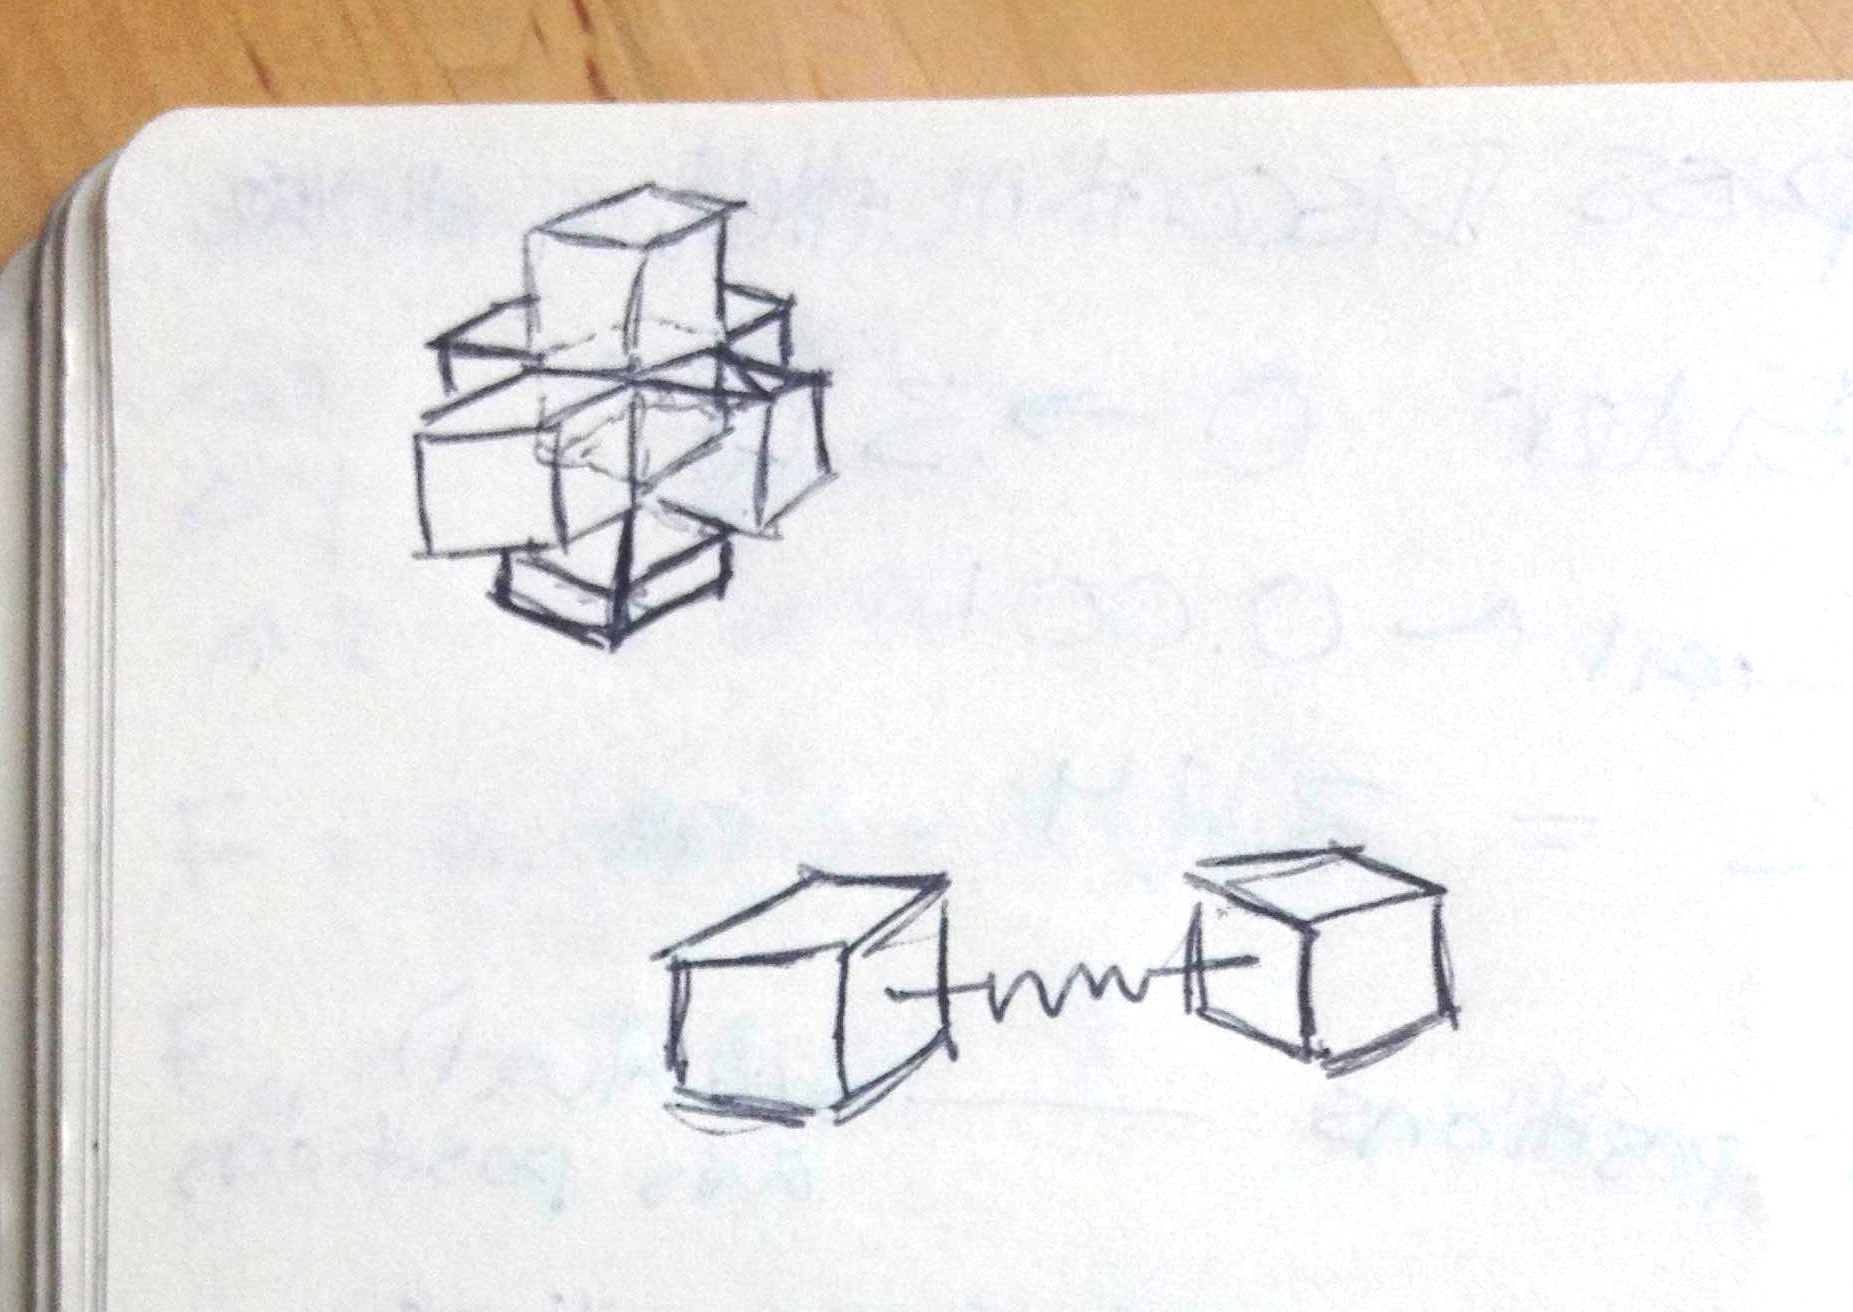
\includegraphics[width=\linewidth]{helloWorldLocalInteraction.png}
  \caption{REPLACE THIS Each cell is face-connected to its six local neighbors \textbf{(A)}.  Interaction between neighbors is modeled with springs constraining translational and rotational motion \textbf{(B)}.  Spring stiffness is determined from material properties of joined cells.}
  \label{fig: helloWorldLocalInteraction}
\end{figure}

\begin{figure}
  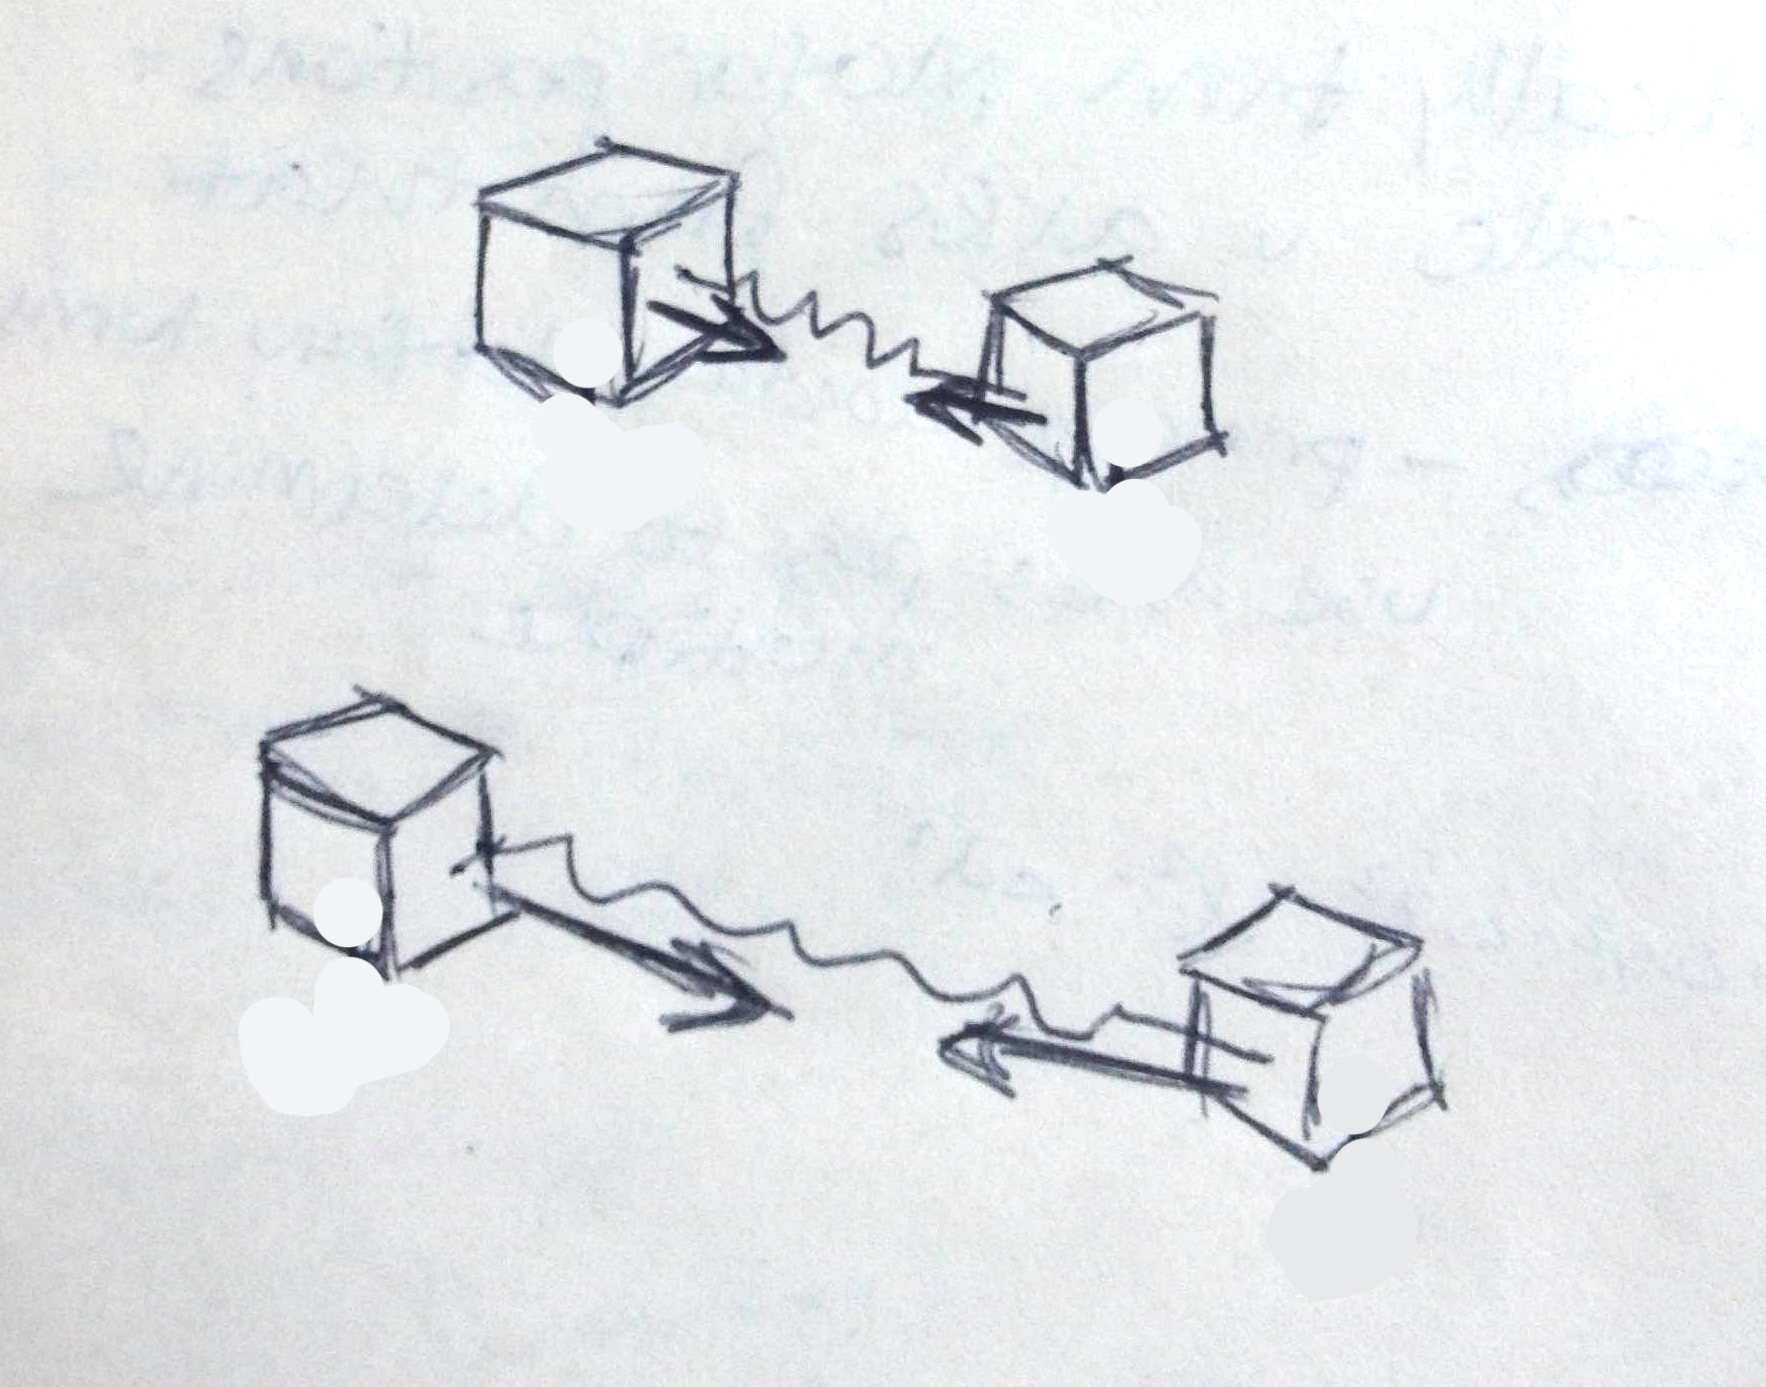
\includegraphics[width=\linewidth]{helloWorldSpring.png}
  \caption{REPLACE THIS Total forces acting on each cell include the force of gravity and the force of all neighboring spring constraints \textbf{(A)}. Larger translational and rotational displacements between neighboring cells increase the amplitude of spring forces \textbf{(B)}.}
  \label{fig: helloWorldSpring}
\end{figure}

To understand how the translational spring forces were calculated between two adjacent cells, consider the 2D case illustrated in Fig \ref{fig: helloWorldSpringSetup}.  The cells are attached by a spring with nominal length $\ell$.  Under displacement $\Delta x$ and $\Delta y$, the total displacement vector from cell A to cell B is given by $\vec{D}$.  Then $\vec{f}$, the force on cell A exerted by the spring, is given by:\\

\[ \vec{f} =  \frac{\vec{D}}{\|D\|} \|f\| = \hat{D} \|f\|\]

where:

\[ \|f\| = \|D\| - \ell\]

then:

\[ \vec{f} = \hat{D} (\|D\| - \ell)\]



\begin{figure}
  \includegraphics[width=\linewidth]{helloWorldSpringSetup.png}
  \caption{REPLACE THIS }
  \label{fig: helloWorldSpringSetup}
\end{figure}





}
